\documentclass[letterpaper, 12pt]{article}

\usepackage{graphicx}
\usepackage{fancyhdr}
\usepackage[T1]{fontenc}
\usepackage{lmodern}
\usepackage[francais]{babel}
%\usepackage[frenchb]{babel}
%\usepackage[applemac]{inputenc}
\usepackage{lipsum}
\usepackage{vmargin}
\usepackage{lastpage}
\usepackage{enumerate}
\usepackage{pdfpages}
\usepackage[nogin]{Sweave}
\usepackage{lscape}
\usepackage{color}
\usepackage{listings}
\usepackage{verbatim}
\usepackage{amssymb, amsmath}
\usepackage{wrapfig}
\usepackage{hyperref}
\usepackage[all]{hypcap}


\begin{document}

\begin{titlepage}
\vspace*{3cm}
\begin{center}

\huge{\bf Types of relation between \\ a variable and its probabilities}\\

\vspace*{2cm}
\large{By Benoit Bruneau}
\end{center}
\vspace*{4cm}

%\hangindent=1cm
%\begin{flushleft}
\begin{description}
\item[Package:] `bmisc'
\item[Version:] 0.2-12
\item[Depends:] car, lattice, zoo, robustbase, and methods
\item[Author \& Maintainer:] Benoit Bruneau (\href{mailto:benoit.bruneau1@gmail.com}{benoit.bruneau1@gmail.com})
\item[Description:] These functions can be used to estimate probabilities \verb=[0,1]= by specifying the inflection points of a relation. Described relations are of type `const', `full', `ramp' and `logistic'.
\item[License:] LGPL $\geqslant$ 3.0
\end{description}


\vspace*{\fill;}


\end{titlepage}

\tableofcontents
\newpage

\section{Types `const', `full', and `plat.full'}
\noindent These relations are the simplest that can be used. While `const' stands for a constant probability of one for all 
values of \verb#x# (Figure~\ref{fig1}), the other two have "all-or-nothing" types of probabilities. One or two thresholds 
(inflection points) need to be defined for types `full' and `plat.full'. The main difference between `full'
(Figure~\ref{fig2} \& \ref{fig3} ) 
and `plat.full' (Figure~\ref{fig4}, \ref{fig5} \& \ref{fig6}) types are the number of thresholds. For all types, `plat' stands for "plateau".\\*

\begin{description}
\item[const.sel]\verb#(x)#
\item[full.sel]\verb#(x, infl1, neg=FALSE, lv=0, uv=1)#
\item[plat.full.sel]\verb#(x, infl1, infl2, neg=FALSE, lv=c(0,0), uv=c(1,1))#
\end{description}
where \verb#infl1# and \verb#infl2# are the inflection points, \verb#x# is a numeric vector for which probabilities are 
estimated, \verb#neg# indicates if the trend is negative  (\verb#TRUE#) or positive (\verb#FALSE#), \verb#lv# defines the 
lower probability values of the relation, and \verb#uv# defines the upper probability values of the relation. By default, 
all fonctions have \verb#neg=FALSE#, \verb#lv=c(0,0)#, and \verb#uv=c(1,1)#.\\*

Here is an example for `const' type:


\begin{Schunk}
\begin{Sinput}
> data = 0:3000
> const.sel(x = data)
\end{Sinput}
\end{Schunk}

\begin{figure}[h]
\vspace{-20pt}
\begin{center}
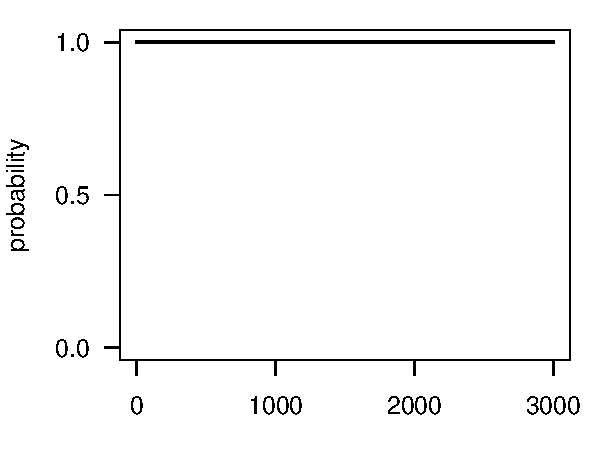
\includegraphics{relation_sel-003}
\end{center}
  \vspace{-30pt}
  \caption{Type `const' probabilities.}
  \vspace{-10pt}
\label{fig1}
\end{figure}
\vspace*{\fill;}

%%%%%%%%%%%%%%%%%%%%%%%%%%%%%%%%%%%%%%%%%%%%%%%%%%%%%%%%%%%%%%%%%%%%%%%%%%%%%%%%%%%%%%%%%%%%%%%%%%%

\newpage

Here are examples for `full' type:
\begin{Schunk}
\begin{Sinput}
> data = 0:3000
> full.sel(x = data, infl1 = 1500, neg = FALSE)
> full.sel(x = data, infl1 = 1500, neg = TRUE)
\end{Sinput}
\end{Schunk}

\begin{figure}[h]
\vspace{-20pt}
\begin{center}
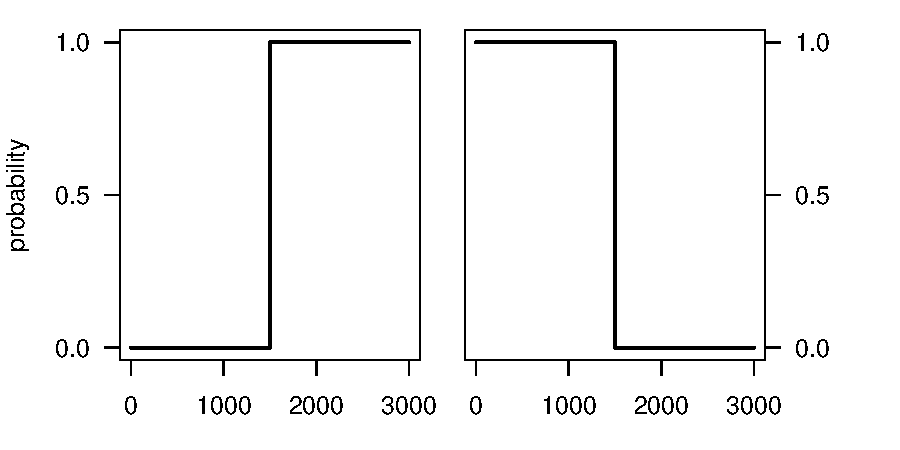
\includegraphics{relation_sel-005}
\end{center}
\vspace{-30pt}
\caption{Type `full' probabilities (left -> neg=FALSE |  right -> neg=TRUE).}
\vspace{-10pt}
\label{fig2}
\end{figure}

\begin{Schunk}
\begin{Sinput}
> data = 0:3000
> full.sel(x = data, infl1 = 1500, neg = FALSE, lv = 0.2, uv = 0.8)
> full.sel(x = data, infl1 = 1500, neg = TRUE, lv = 0.2, uv = 0.8)
\end{Sinput}
\end{Schunk}

\begin{figure}[h]
\vspace{-20pt}
\begin{center}
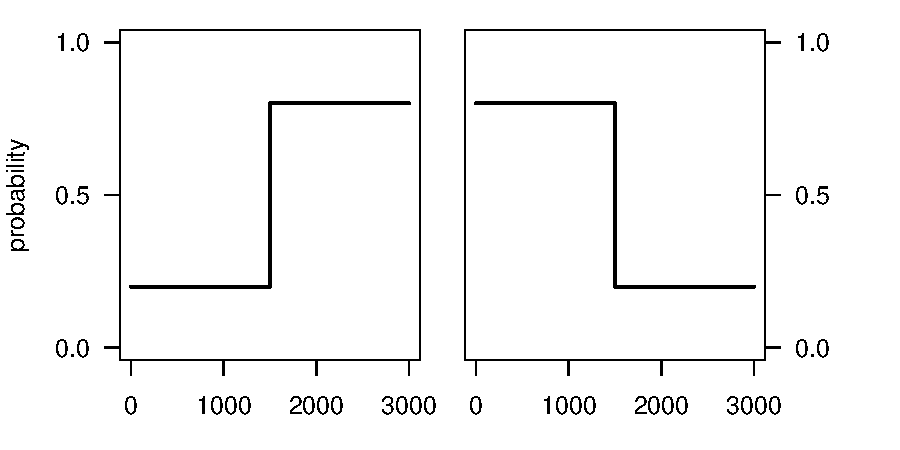
\includegraphics{relation_sel-007}
\end{center}
\vspace{-30pt}
\caption{Type `full' probabilities (left -> neg=FALSE |  right -> neg=TRUE). In this example, minimum and maximum probabilities are respectively lv=0.2 and uv=0.8.}
\vspace{-10pt}
\label{fig3}
\end{figure}

%%%%%%%%%%%%%%%%%%%%%%%%%%%%%%%%%%%%%%%%%%%%%%%%%%%%%%%%%%%%%%%%%%%%%%%%%%%%%%%%%%%%%%%%%%%%%%%%%%%
\newpage
Here are examples for `plat.full' type:
\begin{Schunk}
\begin{Sinput}
> data = 0:3000
> plat.full.sel(x = data, infl1 = 1000, infl2 = 2000, neg = FALSE)
> plat.full.sel(x = data, infl1 = 1000, infl2 = 2000, neg = TRUE)
\end{Sinput}
\end{Schunk}
\begin{figure}[h]
\vspace{-20pt}
\begin{center}
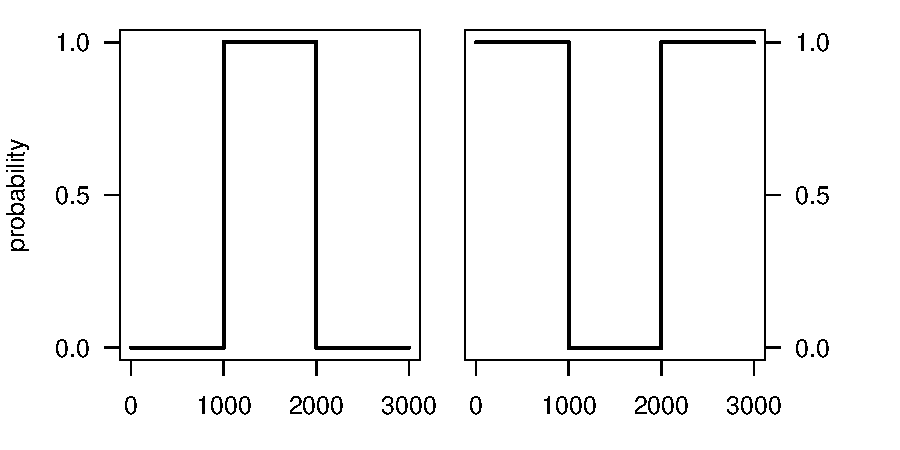
\includegraphics{relation_sel-009}
\end{center}
\vspace{-30pt}
\caption{Type `plat.full' probabilities (left -> neg=FALSE |  right -> neg=TRUE).}
\vspace{-10pt}
\label{fig4}
\end{figure}



\begin{Schunk}
\begin{Sinput}
> data = 0:3000
> plat.full.sel(x = data, infl1 = 1000, infl2 = 2000, neg = FALSE, 
+     lv = 0.2, uv = 0.8)
> plat.full.sel(x = data, infl1 = 1000, infl2 = 2000, neg = TRUE, 
+     lv = 0.2, uv = 0.8)
\end{Sinput}
\end{Schunk}
\begin{figure}[h]
\vspace{-20pt}
\begin{center}
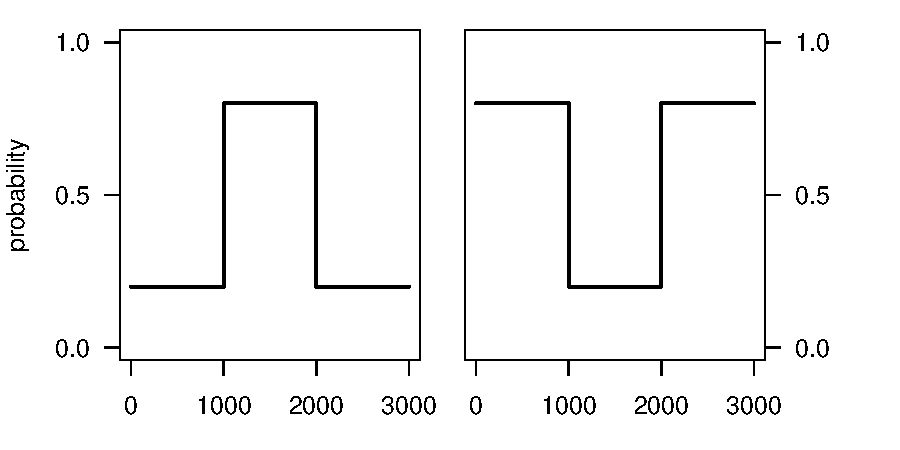
\includegraphics{relation_sel-011}
\end{center}
\vspace{-30pt}
\caption{Type `plat.full' probabilities (left -> neg=FALSE |  right -> neg=TRUE). In this example, minimum and maximum probabilities are respectively lv=0.2 and uv=0.8.}
\vspace{-10pt}
\label{fig5}
\end{figure}

\begin{Schunk}
\begin{Sinput}
> data = 0:3000
> plat.full.sel(x = data, infl1 = 1000, infl2 = 2000, neg = FALSE, 
+     lv = c(0.2, 0.4), uv = 0.8)
> plat.full.sel(x = data, infl1 = 1000, infl2 = 2000, neg = TRUE, 
+     lv = 0.2, uv = c(0.8, 0.6))
\end{Sinput}
\end{Schunk}
\begin{figure}[h]
\vspace{-20pt}
\begin{center}
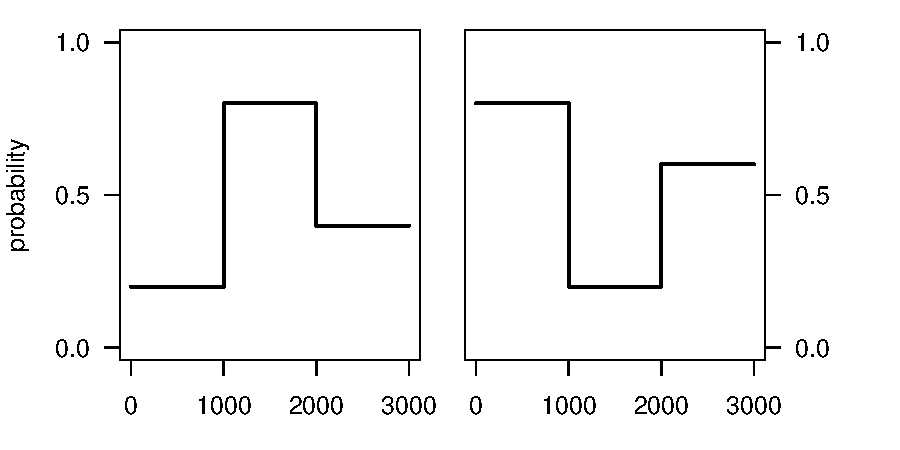
\includegraphics{relation_sel-013}
\end{center}
\vspace{-30pt}
\caption{Type `plat.full' probabilities (left -> neg=FALSE, lv=c(0.2,0.4) , uv=0.8 | right -> neg=TRUE, lv=0.2, uv=c(0.8,0.6)).}
\vspace{-10pt}
\label{fig6}
\end{figure}


%%%%%%%%%%%%%%%%%%%%%%%%%%%%%%%%%%%%%%%%%%%%%%%%%%%%%%%%%%%%%%%%%%%%%%%%%%%%%%%%%%%%%%%%%%%%%%%%%%%

\newpage

\section{Types `ramp' and `plat.ramp'}
\noindent These relations involve adding a gradual increase (or decrease) of probabitily between two inflection points. 
They are an 'upgraded' version of `full' and `plat.full'. Two or four inflection points are needed. 
The main difference between `ramp'(Figure \ref{fig7} \& \ref{fig8}) and `plat.ramp' (Figure \ref{fig9}, \ref{fig10} \& \ref{fig11}) 
types are the number inflection points.\\*
			
\begin{description}
\item[ramp.sel]\verb#(x, infl1, infl2, neg=FALSE, lv=0, uv=1)#
\item[plat.ramp.sel]\verb#(x, infl1, infl2, infl3, infl4, neg=FALSE,# \\* \verb#lv=c(0,0), uv=c(1,1))#
\end{description}
where \verb#infl1# to \verb#infl4# are the inflection points, \verb#x# is a numeric vector for which probabilities are 
estimated, \verb#neg# indicates if the trend is negative  (\verb#TRUE#) or positive (\verb#FALSE#), \verb#lv# defines the 
lower probability values of the relation, and \verb#uv# defines the upper probability values of the relation. By default, 
all fonctions have \verb#neg=FALSE#, \verb#lv=c(0,0)#, and \verb#uv=c(1,1)#.\\*

Here are examples for `ramp' type:
\begin{Schunk}
\begin{Sinput}
> ramp.sel(x = data, infl1 = 1000, infl2 = 2000, neg = FALSE)
> ramp.sel(x = data, infl1 = 1000, infl2 = 2000, neg = TRUE)
\end{Sinput}
\end{Schunk}

\begin{figure}[h]
\vspace{-20pt}
\begin{center}
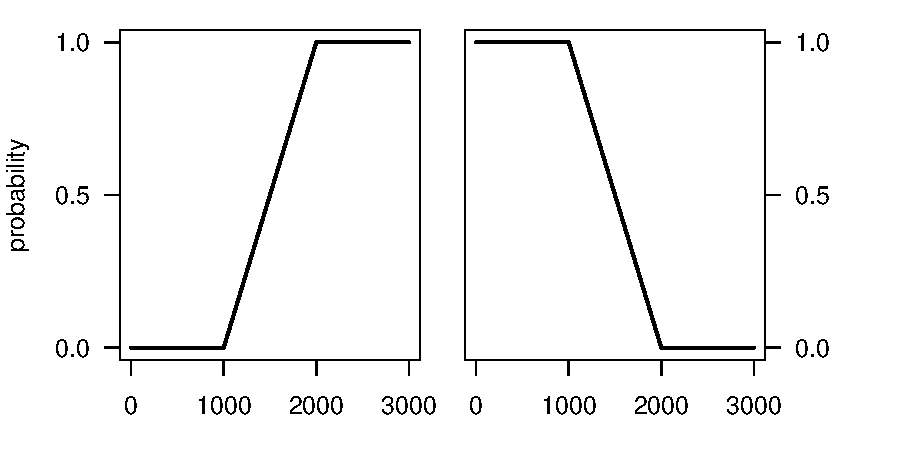
\includegraphics{relation_sel-015}
\end{center}
\vspace{-30pt}
\caption{Type 'ramp' probabilities (left -> neg=FALSE |  right -> neg=TRUE).}
\vspace{-10pt}
\label{fig7}
\end{figure}

\vspace*{\fill;}
\newpage


\begin{Schunk}
\begin{Sinput}
> ramp.sel(x = data, infl1 = 1000, infl2 = 2000, neg = FALSE, lv = 0.2, 
+     uv = 0.8)
> ramp.sel(x = data, infl1 = 1000, infl2 = 2000, neg = TRUE, lv = 0.2, 
+     uv = 0.8)
\end{Sinput}
\end{Schunk}

\begin{figure}[h]
\vspace{-20pt}
\begin{center}
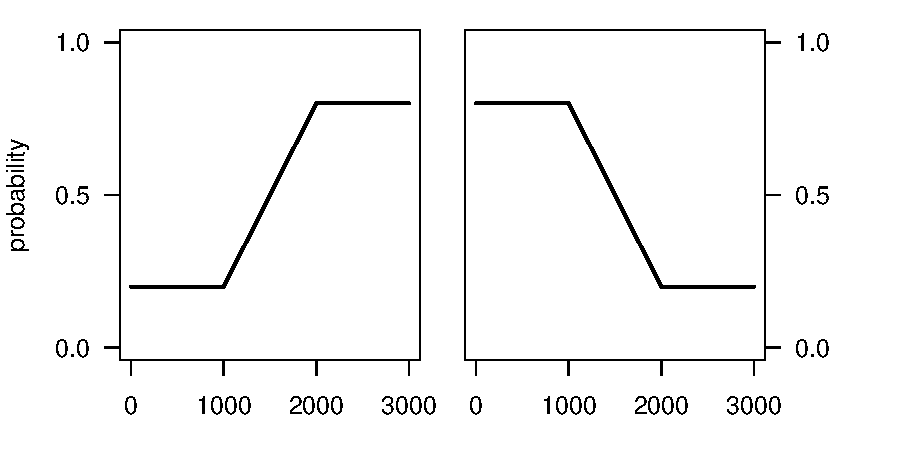
\includegraphics{relation_sel-017}
\end{center}
\vspace{-30pt}
\caption{Type 'ramp' probabilities (left -> neg=FALSE |  right -> neg=TRUE). In this example, minimum and maximum probabilities are respectively lv=0.2 and uv=0.8.}
\vspace{-10pt}
\label{fig8}
\end{figure}



\begin{Schunk}
\begin{Sinput}
> data = 0:3000
> plat.ramp.sel(x = data, infl1 = 500, infl2 = 1000, infl3 = 2000, 
+     infl4 = 2500, neg = FALSE)
> plat.ramp.sel(x = data, infl1 = 500, infl2 = 1000, infl3 = 2000, 
+     infl4 = 2500, neg = TRUE)
\end{Sinput}
\end{Schunk}
\begin{figure}[h]
\vspace{-20pt}
\begin{center}
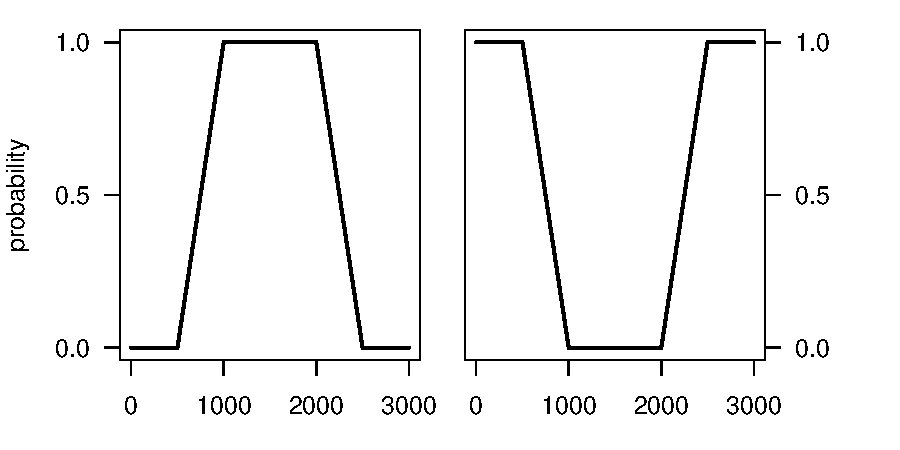
\includegraphics{relation_sel-019}
\end{center}
\vspace{-30pt}
\caption{Type 'plat.ramp' probabilities (left -> neg=FALSE |  right -> neg=TRUE).}
\vspace{-10pt}
\label{fig9}
\end{figure}


\begin{Schunk}
\begin{Sinput}
> data = 0:3000
> plat.ramp.sel(x = data, infl1 = 500, infl2 = 1000, infl3 = 2000, 
+     infl4 = 2500, neg = FALSE, lv = 0.2, uv = 0.8)
> plat.ramp.sel(x = data, infl1 = 500, infl2 = 1000, infl3 = 2000, 
+     infl4 = 2500, neg = TRUE, lv = 0.2, uv = 0.8)
\end{Sinput}
\end{Schunk}
\begin{figure}[h]
\vspace{-20pt}
\begin{center}
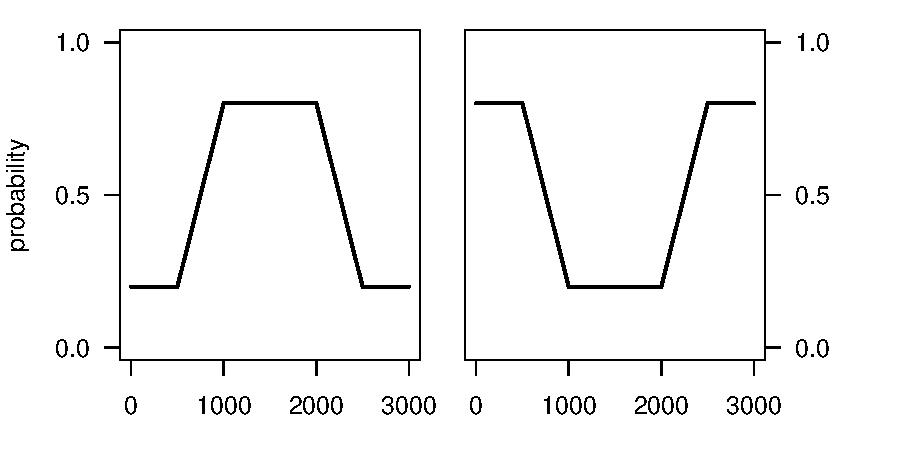
\includegraphics{relation_sel-021}
\end{center}
\vspace{-30pt}
\caption{Type 'plat.ramp' probabilities (left -> neg=FALSE |  right -> neg=TRUE). In this example, minimum and maximum probabilities are respectively lv=0.2 and uv=0.8.}
\vspace{-20pt}
\label{fig10}
\end{figure}

\begin{Schunk}
\begin{Sinput}
> data = 0:3000
> plat.ramp.sel(x = data, infl1 = 500, infl2 = 1000, infl3 = 2000, 
+     infl4 = 2500, neg = FALSE, lv = c(0.2, 0.4), uv = 0.8)
> plat.ramp.sel(x = data, infl1 = 500, infl2 = 1000, infl3 = 2000, 
+     infl4 = 2500, neg = TRUE, lv = 0.2, uv = c(0.8, 0.6))
\end{Sinput}
\end{Schunk}
\begin{figure}[h]
\vspace{-20pt}
\begin{center}
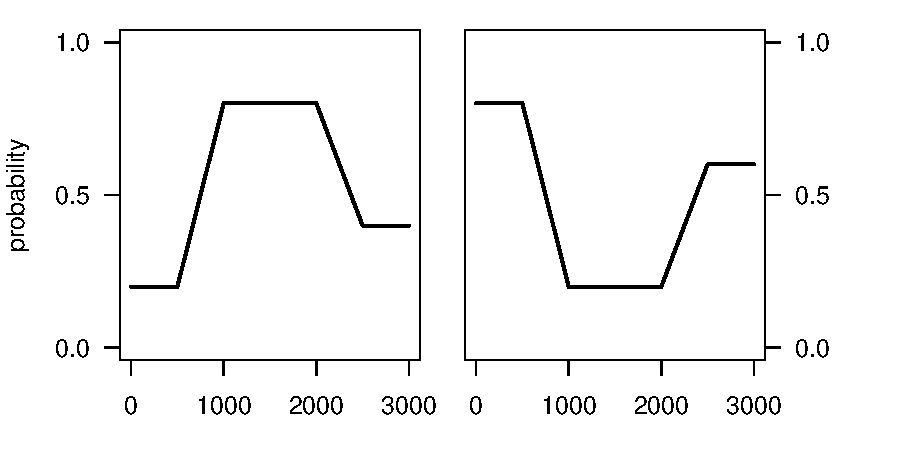
\includegraphics{relation_sel-023}
\end{center}
\vspace{-30pt}
\caption{Type 'plat.ramp' probabilities (left -> neg=FALSE, lv=c(0.2,0.4) , uv=0.8 | right -> neg=TRUE, lv=0.2, uv=c(0.8,0.6)).}
\vspace{-10pt}
\label{fig11}
\end{figure}

%%%%%%%%%%%%%%%%%%%%%%%%%%%%%%%%%%%%%%%%%%%%%%%%%%%%%%%%%%%%%%%%%%%%%%%%%%%%%%%%%%%%%%%%%%%%%%%%%%%
\newpage

\section{Types `logit' and `plat.logit'}
\noindent These relations use logistic curves. Inflection points are defined as points where the intantaneous splope 
is a proportion (\verb#prop#) of the intantenuous slope at $x_{50}$. These types make use of the function \verb#find.beta()# 
of \verb#package::bmisc#. Default value of \verb#prop# is \verb#0.1#. The end result is a logistic curve with 
$x_{50}$ being the midpoint between the inflection points. Two or four inflection points are needed. 
The main difference between `logit'(Figure \ref{fig12} \& \ref{fig13}) and `plat.logit' (Figure \ref{fig14}, \ref{fig15} \& \ref{fig16}) 
types are the number inflection points.\\*

\begin{description}
\item[logit.sel]\verb#(x, infl1, infl2, neg=FALSE, lv=0, uv=1, ...)#
\item[plat.logit.sel]\verb#(x, infl1, infl2, infl3, infl4, neg=FALSE,# \\* \verb#lv=c(0,0), uv=c(1,1), ...)#
\end{description}
where \verb#infl1# to \verb#infl4# are the inflection points, \verb#x# is a numeric vector for which probabilities are 
estimated, \verb#neg# indicates if the trend is negative  (\verb#TRUE#) or positive (\verb#FALSE#), \verb#lv# defines the 
lower probability values of the relation, and \verb#uv# defines the upper probability values of the relation. By default, 
all fonctions have \verb#neg=FALSE#, \verb#lv=c(0,0)#, and \verb#uv=c(1,1)#. Additionnal options of \verb#find.beta()# 
can be added. Default values are \verb#prob=NULL#, \verb#prop=0.1#,\verb#beta=0.2#, and \verb#fast=TRUE#.  \\*

Here are examples for these types:
\begin{Schunk}
\begin{Sinput}
> logit.sel(x = data, infl1 = 1000, infl2 = 2000, neg = FALSE)
> logit.sel(x = data, infl1 = 1000, infl2 = 2000, neg = TRUE)
\end{Sinput}
\end{Schunk}
\begin{figure}[h]
\vspace{-20pt}
\begin{center}
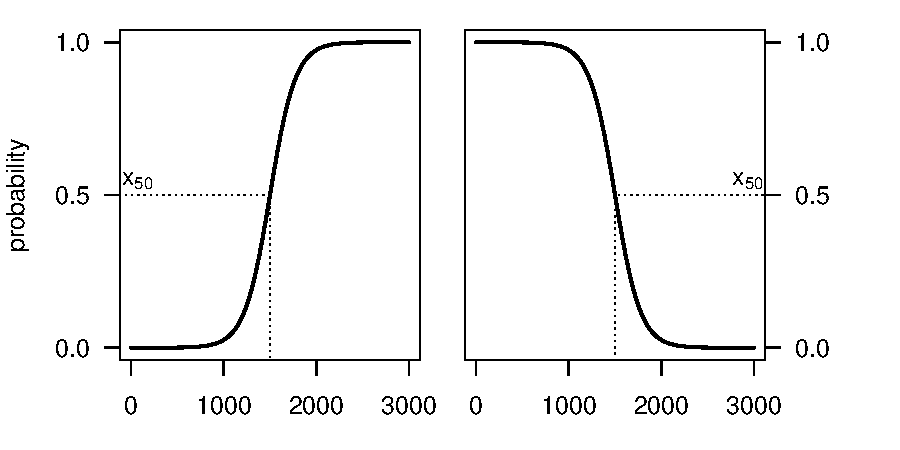
\includegraphics{relation_sel-025}
\end{center}
\vspace{-30pt}
\caption{Type 'logit' probabilities (left -> neg=FALSE |  right -> neg=TRUE).}
\vspace{-10pt}
\label{fig12}
\end{figure}

\vspace*{\fill;}
\newpage


\begin{Schunk}
\begin{Sinput}
> logit.sel(x = data, infl1 = 1000, infl2 = 2000, neg = FALSE, 
+     lv = 0.2, uv = 0.8)
> logit.sel(x = data, infl1 = 1000, infl2 = 2000, neg = TRUE, lv = 0.2, 
+     uv = 0.8)
\end{Sinput}
\end{Schunk}

\begin{figure}[h]
\vspace{-20pt}
\begin{center}
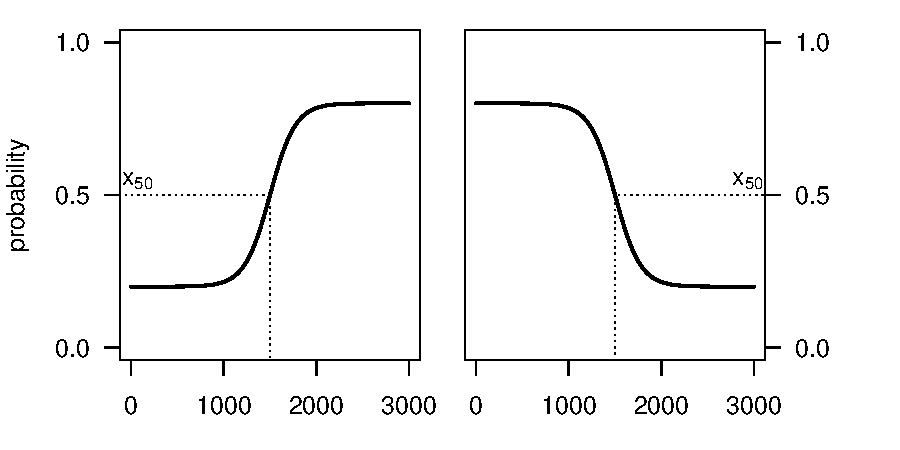
\includegraphics{relation_sel-027}
\end{center}
\vspace{-30pt}
\caption{Type 'logit' probabilities (left -> neg=FALSE |  right -> neg=TRUE). In this example, minimum and maximum probabilities are respectively lv=0.2 and uv=0.8.}
\vspace{-10pt}
\label{fig13}
\end{figure}



\begin{Schunk}
\begin{Sinput}
> data = 0:3000
> plat.logit.sel(x = data, infl1 = 500, infl2 = 1000, infl3 = 2000, 
+     infl4 = 2500, neg = FALSE)
> plat.logit.sel(x = data, infl1 = 500, infl2 = 1000, infl3 = 2000, 
+     infl4 = 2500, neg = TRUE)
\end{Sinput}
\end{Schunk}
\begin{figure}[h]
\vspace{-20pt}
\begin{center}
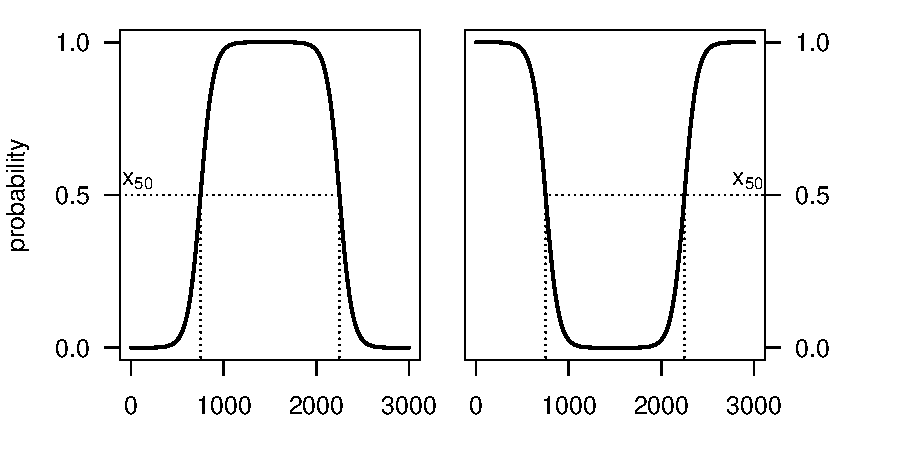
\includegraphics{relation_sel-029}
\end{center}
\vspace{-30pt}
\caption{Type 'plat.logit' probabilities (left -> neg=FALSE |  right -> neg=TRUE).}
\vspace{-10pt}
\label{fig14}
\end{figure}


\begin{Schunk}
\begin{Sinput}
> data = 0:3000
> plat.logit.sel(x = data, infl1 = 500, infl2 = 1000, infl3 = 2000, 
+     infl4 = 2500, neg = FALSE, lv = 0.2, uv = 0.8)
> plat.logit.sel(x = data, infl1 = 500, infl2 = 1000, infl3 = 2000, 
+     infl4 = 2500, neg = TRUE, lv = 0.2, uv = 0.8)
\end{Sinput}
\end{Schunk}
\begin{figure}[h]
\vspace{-20pt}
\begin{center}
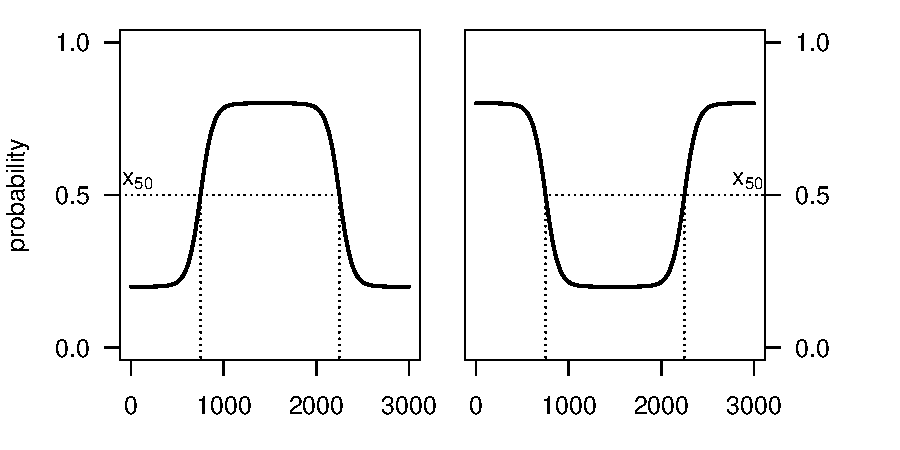
\includegraphics{relation_sel-031}
\end{center}
\vspace{-30pt}
\caption{Type 'plat.logit' probabilities (left -> neg=FALSE |  right -> neg=TRUE). In this example, minimum and maximum probabilities are respectively lv=0.2 and uv=0.8.}
\vspace{-20pt}
\label{fig15}
\end{figure}

\begin{Schunk}
\begin{Sinput}
> data = 0:3000
> plat.logit.sel(x = data, infl1 = 500, infl2 = 1000, infl3 = 2000, 
+     infl4 = 2500, neg = FALSE, lv = c(0.2, 0.4), uv = 0.8)
> plat.logit.sel(x = data, infl1 = 500, infl2 = 1000, infl3 = 2000, 
+     infl4 = 2500, neg = TRUE, lv = 0.2, uv = c(0.8, 0.6))
\end{Sinput}
\end{Schunk}
\begin{figure}[h]
\vspace{-20pt}
\begin{center}
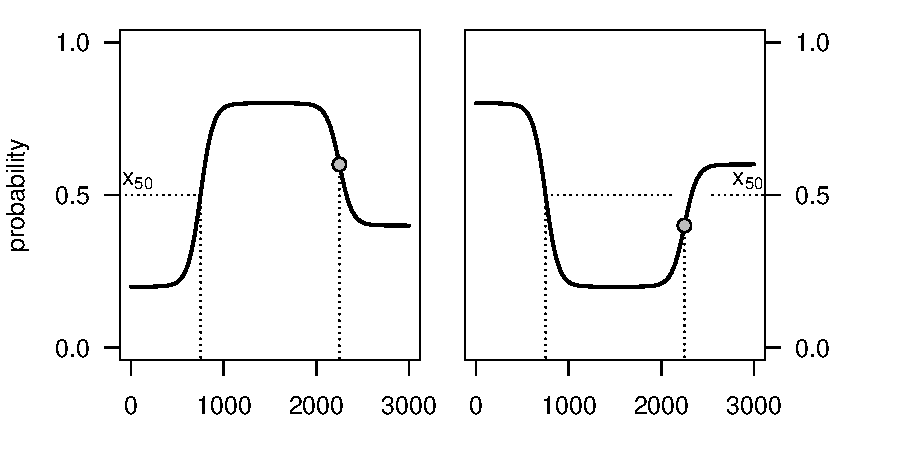
\includegraphics{relation_sel-033}
\end{center}
\vspace{-30pt}
\caption{Type 'plat.logit' probabilities (left -> neg=FALSE, lv=c(0.2,0.4) , uv=0.8 | right -> neg=TRUE, lv=0.2, uv=c(0.8,0.6)).}
\vspace{-10pt}
\label{fig16}
\end{figure}







        
        
\end{document}
